\subsection{Methodology}

After the dataset creation ...

The end of each Karoo GP training produces a multivariate exression with heighest fitness score. We repeat the training process 200 times to get 200 expressions for each label (hasNS and hasRemnant). Due to the stochastic nature of the GP algorithm, the expressions mostly tend to be unique depending upon the complexity of the classification problem. Each expression can then be used to classify the reconstructed source parameters to determine the labels hasNS and hasRemnant by substituting the values in the expression. If the result is greater or equal to zero, we classify the reconsturcted set of prameter as true and false otherwise. The performace of each of the expressions against the testing set for one EoS is shown in Fig \ref{fig:FPR_TPR}. As seen in the plots, the average performace of hasRemnant expressions is better than hasNS expressions. Also the winning expressions are more dispersed in case of hasRemnant.  

\begin{figure*}[htp]
  \centering
  \subfloat[]{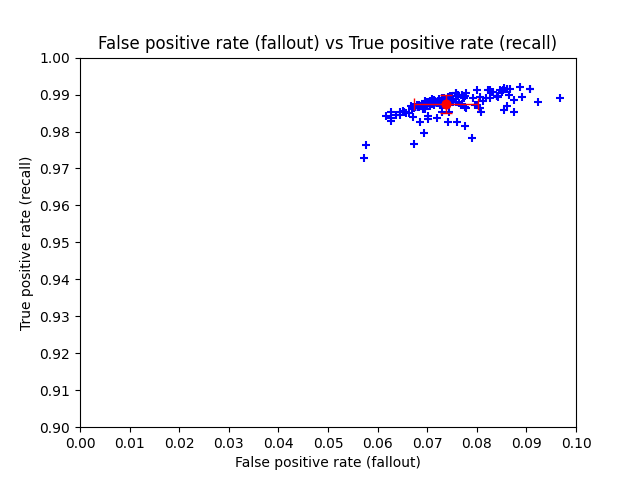
\includegraphics[scale=0.5]{plots/FPR_TPR/FPR_TPR_NS_MS1_PP.png}}\quad
  \subfloat[]{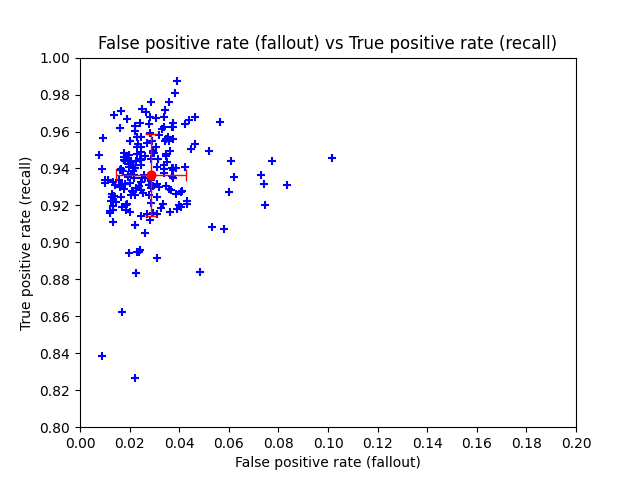
\includegraphics[scale=0.5]{plots/FPR_TPR/FPR_TPR_EMB_MS1_PP.png}}
  \caption{The plot on the left is a FPR (False Positive Rate) vs (True Positive Rate) plot for all 200 winning expressions for hasNS classification on MS1_PP EoS. The red dot is the average of TPR and FPR of the expressions and the vetricle and horizontal spread are the one sigma values for TPR and FPR respectively. The plot on the right is similar but for hasRemnant classification.  }
  \label{fig:FPR_TPR}
\end{figure*}

